\documentclass[a4paper,12pt]{article}
\usepackage[utf8]{inputenc}
\usepackage{amsmath,amssymb,graphicx}
\usepackage{amsmath,graphicx}
\usepackage{tikz}
\usetikzlibrary{matrix}
\usepackage[a4paper,left=3.5cm, right=3.5cm, top=2.5cm, bottom=2.5cm]{geometry}
\usepackage{hyperref}
\hypersetup{
    colorlinks=true,
    linkcolor=blue,
    filecolor=magenta,      
    urlcolor=cyan,
}

\urlstyle{same}

\title{ \vspace{-50pt} Correlations of crime and land use in Chicago}
\author{Jorge Gerardo Acosta Montes }
\date{}

\begin{document}
\maketitle
\section{Introduction}
This project explores the correlations between the amount and types of crimes committed in a community area and the venues located there.  

Crime is a multi-factorial phenomena, and the study of only one component should acknowledge other variables. In order to have  meaningful comparisons between two or more regions. The relations between crime and socioeconomic conditions are unclear. Often there are contradictory reports on whether difficult economic conditions create more crime or whether a booming economy that increases the availability of money and goods promotes crime. Nevertheless, it is important to do not dismiss possible connections between the economy and crime. In this project, I will try to find if the crimes committed in community areas with similar socioeconomic indicators have a relation with the land use. For example, let's suppose that  A and B are community areas with similar economic conditions, but area A is much safer than area B. I want to see if the types of venues in area A are similar to those in area B. If they are not similar, then study what types of venues are present in the safer environment.  The venues could be parks, liquor shops, restaurants among others. 

Also, venues that reduce or increase crime in one type of area do not necessarily have an impact in crime in other types of areas.  One possible hypothesis is that parks can be that kind of venue. In areas with a high rate of crime, social interactions can induce people to become criminals. Parks promote social interaction.  Therefore parks there contribute to crime. On the other hand, parks will not affect crime in areas with low rate crime. 

This project could help policymakers to design safer neighborhoods by building or closing venues to reduce crime.

\section{Data}
Cultural and geographical factors affect societies in complex ways. A study of crime among different cities with different cultures will need to take in account cultural indicators, and will require a score that already take those indicators to compare to compare two different cities. This is a modest study, and I will dismiss all cultural factors. To reduce the effects of those variables, only  areas in the same city will be considered. Due to the availability of the data, I choose Chicago. The datasets of the crime and economic status of the neighborhoods in Chicago were already given in previous courses of this certification, and were made by the city of Chicago. The socioeconomic data can be downloaded in \url{https://ibm.box.com/shared/static/05c3415cbfbtfnr2fx4atenb2sd361ze.csv}. Crime data can be downloaded from \url{https://ibm.box.com/shared/static/svflyugsr9zbqy5bmowgswqemfpm1x7f.csv}. Detailed explanations of the data can be found in \url{ https://data.cityofchicago.org/Health-Human-Services/Census-Data-Selected-socioeconomic-indicators-in-C/kn9c-c2s2} and \url{ https://data.cityofchicago.org/Public-Safety/Crimes-2001-to-present/ijzp-q8t2}. 

The dataset of socioeconomic indicators contain 9 parameters and divides the city in 77 areas. A description is provided in the ones that are not clear:
\begin{itemize}
\item \textbf{Community area number}
\item \textbf{Community area name}
\item \textbf{Percent of housing crowded:} Percentage of houses with more people than rooms.
\item \textbf{Percent households below poverty:} Percentage of houses with an income less than the federal poverty level. The table contains data from 2008 to 2012. In 2012 it was an income of 23 050 for a family of 4.
\item \textbf{Percent aged 16+ unemployed}
\item \textbf{Percent aged 25+ without high school diploma}
\item \textbf{Percent aged under 18 or over 64}
\item \textbf{Per capita income}
\item \textbf{Hardship index:}It is an score that combines the 6 socioeconomic indicators in this dataset.
\end{itemize}

The dataset about crime contains a wide description of parameters of crime incidents. I only use:
\begin{itemize}
\item \textbf{Primary type}
\item \textbf{Community area number}
\item \textbf{Latitude}
\item \textbf{Longitude}
\end{itemize}

The land use was determined by the venues that are in a community area. The venues were obtained with the Foursquare API. The location of each community area was assigned as the mean latitude and longitude of the crimes commited in that area. For each area, I set a limit of 50 venues and a radius of 500 meters. I obtained 1219 venues. Of this dataset I only use:
\begin{itemize}
\item \textbf{Community area name}
\item \textbf{Venue Category:} Examples include parks, restaurants, bars and recreation centers.
\end{itemize}  

\section{Methodology}
The community areas were clustered by k-means using the economic indicators of the socioeconomic dataset with the exception of the Hardship index, because that index is already a combination of the other parameters. All the indicators but the per capita income are in a percentage form. The per capita income was transformed to a percentage form, in which the 100\% corresponds to the average per capita income in Chicago. 


\begin{figure}[ht]
 \centering
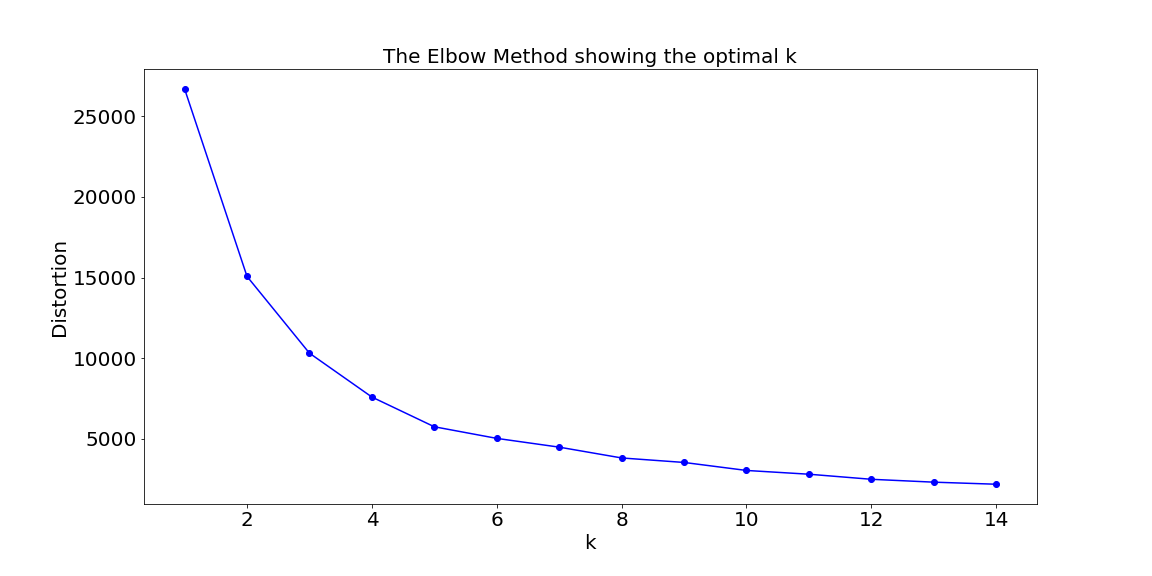
\includegraphics[scale=0.4]{Elbow_method}
\caption{The elbow method shows that 4 is the optimal number of clusters. 
\label{fig:elbow}}
\end{figure} 

The optimal number of clusters was determined using the elbow method, in which the distortion of different numbers of clusters is computed. The distortion is the average distance of the members of a cluster to its center. The numbers of clusters is chosen as the first number after which the distortions follows a linear behavior.


\begin{figure}[!h]
 \centering
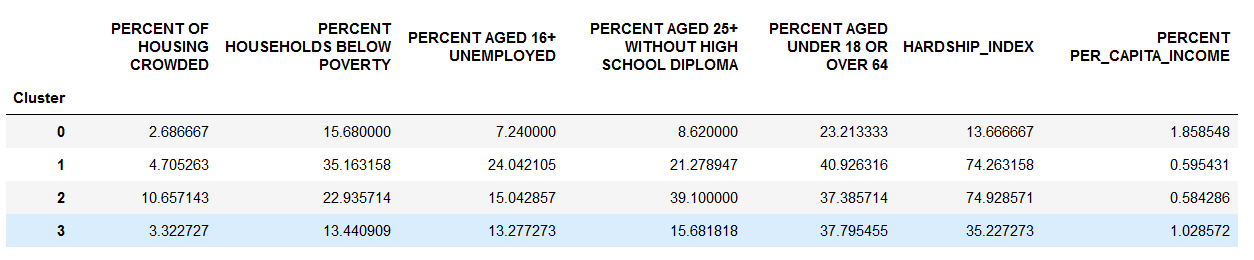
\includegraphics[width=17cm]{economic_indicators_clusters}
\caption{Socioeconomic parameters of the clusters. 
\label{fig:socio_cluster}}
\end{figure} 

The 4 clusters seems to indicate the presence of an upper class, middle class and 2 lower classes, as can be seen in figure \ref{fig:socio_cluster}. Cluster 0 consist of areas with high income, low hardship and good socioeconomical parameters. Clusters 1,2 are poor areas in which the hardship index is high, and the income low. In cluster 1 there are more households in poverty and higher unemployment. Altough the per capita income is slightly higher than in the cluster 2. Cluster 3 represents the middle class. Their average income is close to the average income of the city. 

Cluster 1,2 have a similar socio economical structure but the differences are enough to make them also cluster in terms of locations. A common characteristic in both clusters is the presence of industrial complex. In figure \ref{fig:map_cluster} a map with the location of each community and a color marker indicating its cluster is shown. The geographical information was not considered for the clusters. Nevertheless cluster 0,1,2 also group themselves geographically. The cluster 3 is scattered in all Chicago. The distribution is in accordance with the hypothesis that the cluster represents the middle class. The cluster 0 mainly represent areas within the downtown.


\begin{figure}[hb]
 \centering
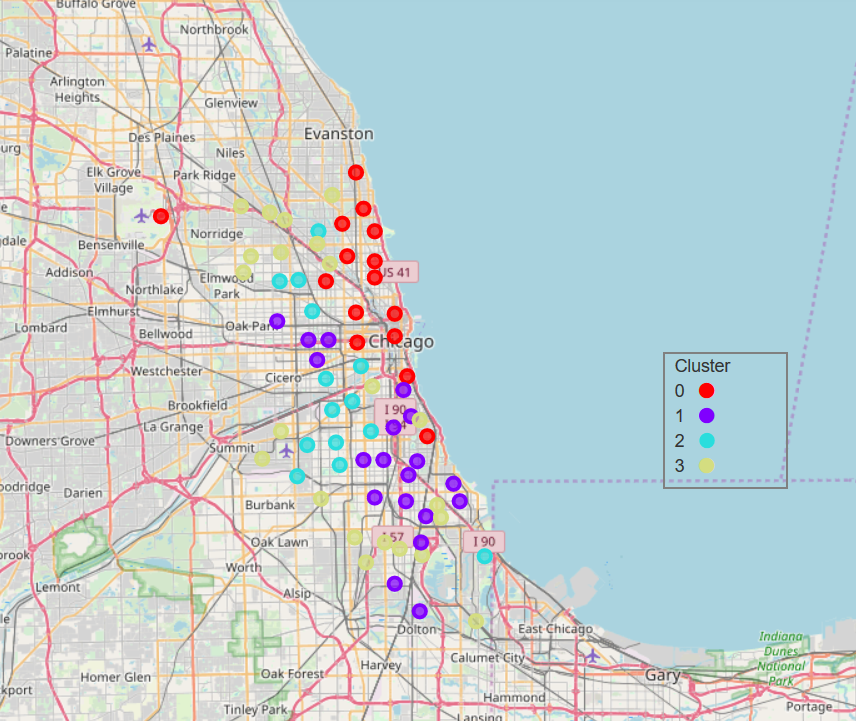
\includegraphics[scale=1]{Cluster_map_chicago}
\caption{Geographical distribution of the clusters. 
\label{fig:map_cluster}}
\end{figure} 

The most common venues per cluster were found \ref{fig:common_venues}, and also the most common crimes per cluster were also found \ref{fig:common_crimes}. The most common venues does not contribute directly to the objective of the project, but it can point possible directions of future studies. Among the 5 most common crimes in each cluster there are 8 categories between all clusters:
\begin{itemize}
\item Theft
\item Battery
\item Crimanl Damage
\item Narcotics
\item Other offense
\item Burglary
\item Assault
\item Deceptive practice

\end{itemize}

\begin{figure}[hb]
 \centering
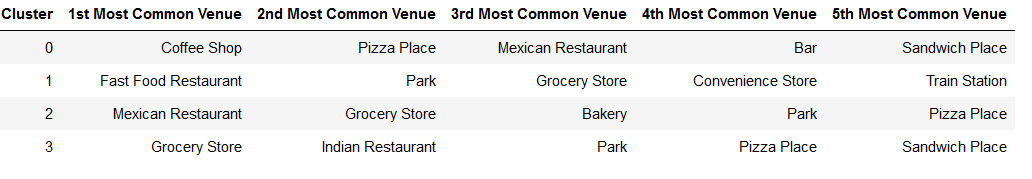
\includegraphics[scale=1]{Common_venues_per_cluster}
\caption{Common venues per cluster. 
\label{fig:common_venues}}
\end{figure}   

\begin{figure}[ht]
 \centering
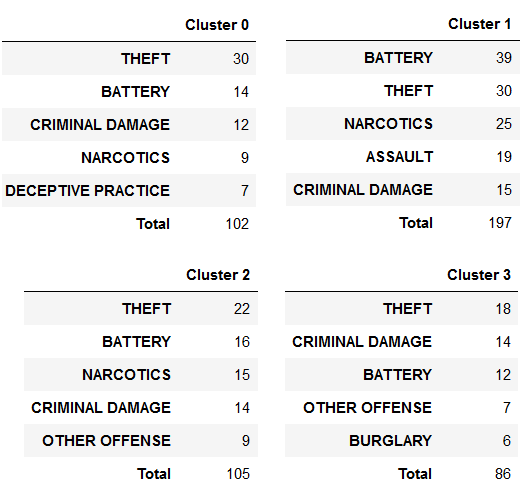
\includegraphics[scale=1]{common_crimes_cluster}
\caption{Common crimes per cluster. 
\label{fig:common_crimes}}
\end{figure}
I will look for correlations between these crimes and the venues located in where these crimes occurred. I dismiss "Other offense" because is vague.

Cluster 1 is clearly the most affected, followed by cluster 2 and 0. A possibility for the high rate of crime in cluster 0 is that there is people with more money there than in the other clusters, therefore it is more attractive to criminals.  

Theft is the most common crime in 3 clusters, and it is the second most common in the other.

I am going to create a heatmap for each cluster. In the heat map,  the "y" axis will be each of the most common crimes and the "x" axis will be venues in which a crime of the most common have a correlation above 0.5 . For example in Theft in the cluster 0, there 4 venues with a correlation above 0.5 these venues will be added to the "x" axis. If there are no venues with a correlation above 0.5 only the venue with the highest correlation will be added. A maximum of 3 venues can be added per crime, this is done to have a small and easier to analyze heatmap.

The heatmap of the cluster 0 is shown in figure \ref{fig:cluster_0}.
\begin{figure}[hb]
 \centering
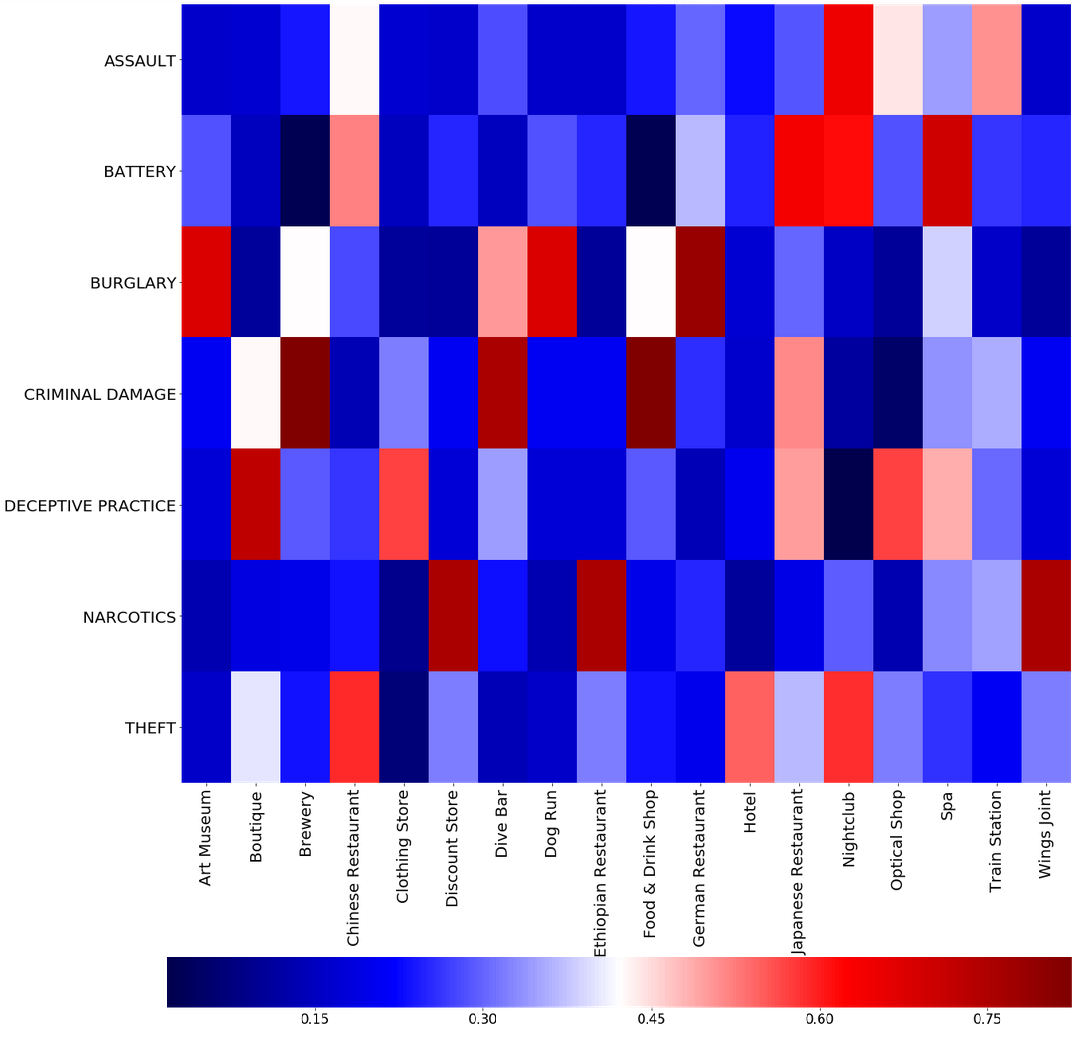
\includegraphics[scale=0.65]{Heatmap_cluster_0}
\caption{Heatmap of cluster 0. 
\label{fig:cluster_0}}
\end{figure}

\section{Results and Discussion}
The correlations between a crime and a venue does not imply causation, but could imply that certain venues promotes crime. In this section, 4 heatmaps of correlations will be presented. Each heatmap correspond to a cluster. The length of the "x" axis is different in each cluster, because the correlations between a venue and crime are different in the clusters, and venues can only be added if a crime in the list of the most commons have a correlation above 0.5 for that venue. Given that there are 7 most common crimes, and a maximum of 3 venues per crime can be added. The maximum length of the "x" axis is 21.

In the heatmap of cluster 0 there are 18 venues which show that the crimes are not strongly related because if one crime implied other, then it could be expected that both crimes would occur in near places. The venue category which is strongly correlated with more crimes is nightclub with 3 crimes: assault, battery and theft. The first two are closely related and the difference is only the severity of the offense. It is not surprising that a nightclub promotes confrontations between people. Considering that cluster 0 is a zone where the upper class lives, the spread in the venues could tells us that the whole zone of cluster 0 is attractive to the crime, and the location and types of venues do not have an impact on the criminal activity in the cluster.
\begin{figure}[hb]
\centering 
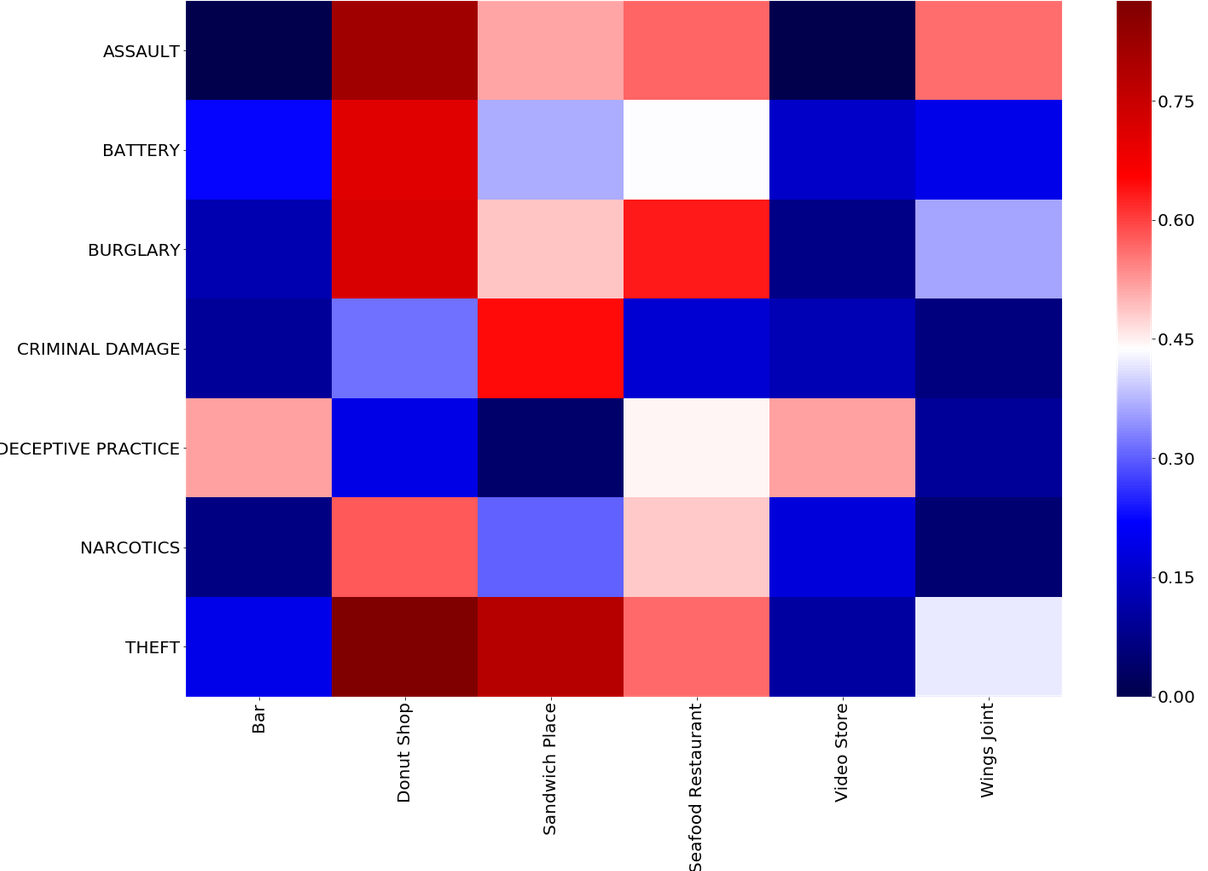
\includegraphics[scale=0.65]{Heatmap_cluster_1} 
\caption{Heatmap of cluster 1. 
\label{fig:cluster_1}} 
\end{figure}

Figure \ref{fig:cluster_1} represent the correlations in the cluster 1. In this case it is the opposite case of the cluster 0. There are only 6 venues. As it can be seen if a crime occurred near a venue is likely that a different crime will occur nearby. The venue category Donut Shop shows a strong correlation with almost all the crimes. I thinks that indicates that the crime is specially localized in a region in which a Donut Shop is located. Also in food places assault, burglary and theft are common. This could indicate that criminals in this cluster look for places where people tend to gather. A police unit near those places could reduce the crime.

The correlations of cluster 2 can be seen in the figure \ref{fig:cluster_2}. In this case there are 11 venues. The venues categories can be classified as food places, recreation places and places where alcohol is sold. In this cluster the presence of a recreation center is negative with respect to crime. There are 4 types of crimes commited in the recreation center: assault, battery, narcotics and theft. In fact it seems that the recreation center act as distribution center of drugs (I am not implying that it is intentional), because it is the only venue with a strong correlation with narcotics. It seems that a crime in a venue does not imply that other crime will be commited in that venue. In this cluster the correlations between crimes and venues are not significant, with the exception of the recreation center.  
\begin{figure}[hb]
\centering 
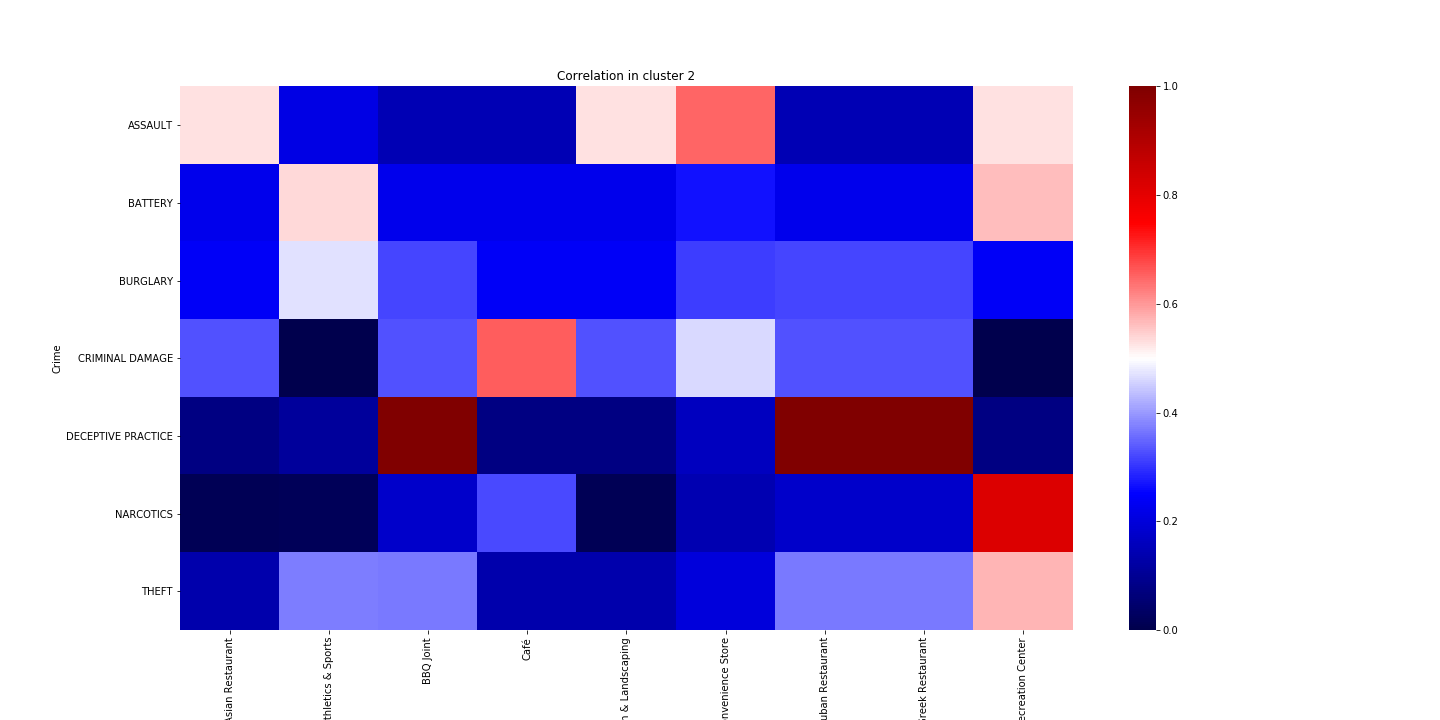
\includegraphics[scale=0.65]{Heatmap_cluster_2} 
\caption{Heatmap of cluster 2. 
\label{fig:cluster_2}} 
\end{figure}

The result of the cluster 3 are shown in figure \ref{fig:cluster_3}. In this cluster there 14 venue categories. This cluster is different in the types of venue categories because there are few venues which are related to food. There are only 2: Café and Food. With the exception of the food related venues, the other venues do not necessarily involve gathering of people.  This cluster have the less amount of crime, see figure \ref{fig:common_crimes}. Theft is the most common crime in this cluster but it seems that is has no relation with the venues, this could indicate that theft is spread along the cluster. It looks that there is a relation between criminal damage, deceptive practice and narcotics in this cluster. When one of those occur in a venue category, it seems that the correlations of the other crimes in that venue category are also significant. Maybe the owner of the venues in which these crimes occur can be warned that it is likely that other criminal activities are taking places near its venues.  

\begin{figure}[hb]
\centering 
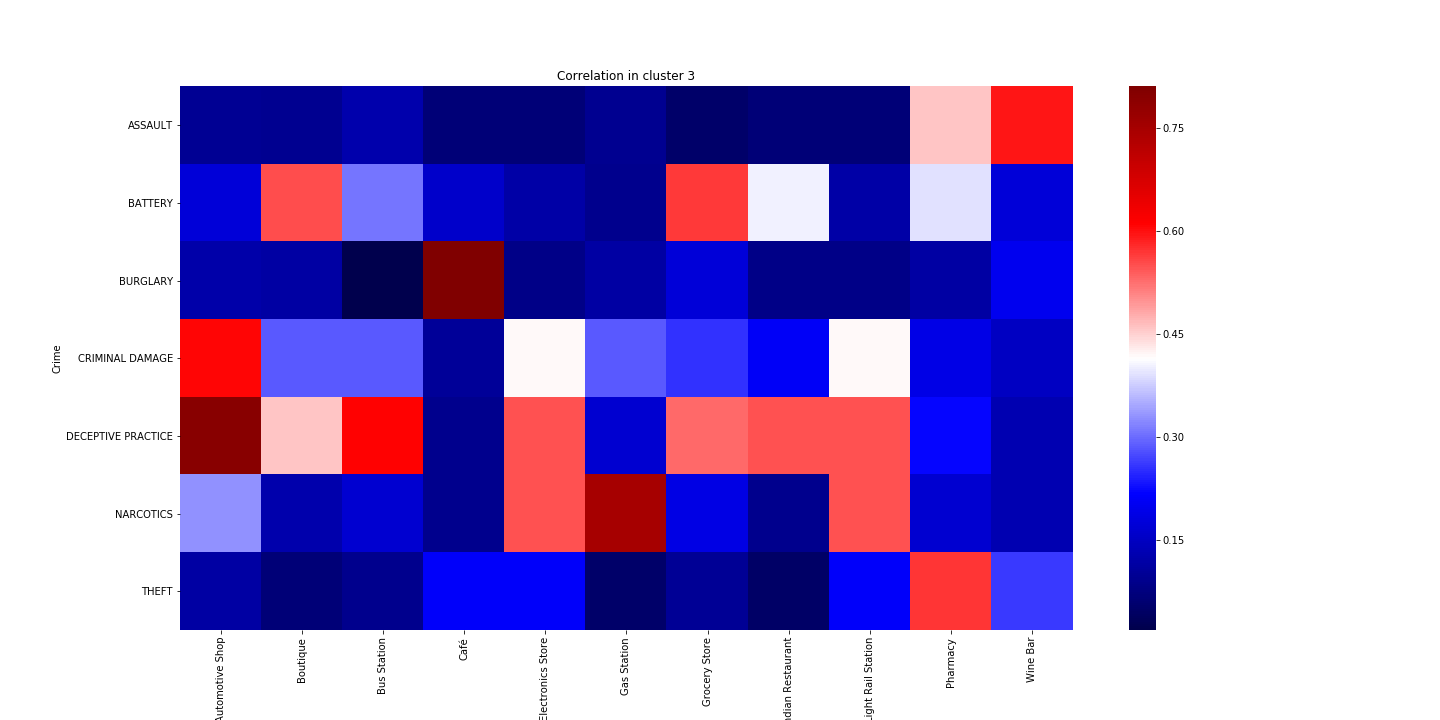
\includegraphics[scale=0.65]{Heatmap_cluster_3} 
\caption{Heatmap of cluster 3. 
\label{fig:cluster_3}} 
\end{figure}

\section{Conclusions and possible future work}
Different cluster experience different amount of crime. The relations between crime and venues is different between clusters. This indicates that the strategies against crime should take into account the socioeconomical status of the communities. In clusters 1,2,3 seems to exist relation between crime and venues. In cluster 0 the crime is distributed among a higher number of venues. In cluster 1 the crime rate is high but it is localized. In cluster 2 the crime only concentrates in the recreation center. A strategy to tackle crime in cluster 3 is not obvious, but a relation among criminal damage, deceptive practice and narcotics should be found to design a better strategy. Luckily, it is the cluster with less crime.

The relation between crime and venues is incomplete if it is not considered where does the criminals live. Criminals that live in one cluster can commit a crime in other cluster, therefore an examination of the venues where the criminals live is necessary. 

    



\end{document}